\chapter{WASI, nel dettaglio}
\label{chap:wasi-in-depth}
L'obiettivo principale di WASI è fornire un set di API standard per WebAssembly, indipendenti dal motore di esecuzione
sottostante. Per raggiungere questo obiettivo è stato necessario creare, in prima istanza, un primo modulo su cui basare
tutti gli altri. Questo modulo è stato chiamato WASI-Core e ha lo scopo di fornire le funzionalità di base per
l'ambiente di esecuzione, come la gestione dei file, delle reti e di essere generico in modo da poter essere utilizzato
in qualsiasi ambiente fuori dal browser. Al di fuori del contesto web, WebAssembly ha bisogno di una serie di API per
interagire con il sistema operativo sottostante, ovvero una libreria di sistema per Wasm. Questa libreria, chiamata
WASI-libc è in grado di fornire un ponte tra i moduli Wasm e le system call del sistema sottostante. È basata sullo
standard POSIX ed in particolare su musl-libc\footnote{\url{http://musl.libc.org/}} ed utilizza le funzioni di
libpreopen\footnote{\url{https://github.com/musec/libpreopen}}.
% È basata sullo standard POSIX in particolare su musl-libc\footnote{\url{http://musl.libc.org/}}, un'implementazione
% dello standard POSIX costruita sulle system call di Linux ed utilizza le funzioni di
% libpreopen\footnote{\url{https://github.com/musec/libpreopen}}, un insieme di funzioni che consente solo l'uso di file
% descriptor già aperti in precedenza, prevenendo così la possibilità di aprire file descriptor direttamente. Questi
% file descriptor sono aperti dai runtime WASI e passati all'applicazione in un secondo momento, in modo da rispettare
% il capability-based security model. L'implementazione di WASI-libc non porta include funzioni come fork() o exec() in
% quanto complesse da sviluppare in ambito sandbox e al momento fuori dallo scope del progetto.

\section{WASI-libc}
WASI-libc\footnote{\url{https://github.com/WebAssembly/WASI/blob/main/legacy/preview1/docs.md}} è una libreria che
definisce un'interfaccia C standard per le system call necessarie a WebAssembly. È il ponte fondamentale che unisce i
moduli Wasm con il sottostante sistema operativo. L'obiettivo chiave della libreria è quello di fornire un set di
funzioni che si comportino come quelle dello standard POSIX, ma che siano implementate specificamente per WebAssembly
tra cui l'allocazione e la manipolazione della memoria, l'I/O dei file, la gestione delle stringhe, le funzioni
matematiche e così via. Essendo un'implementazione personalizzata, non include tutte le funzioni standard di POSIX. Ad
esempio funzioni come la fork() e l'exec() sono escluse in quanto complesse da implementare in ambito sandbox e
difficili da gestire secondo il modello capability-based. La libreria è basata su due altre librerie già esistenti: la
musl-libc e la libpreopen.
\subsection{Musl-libc}
Musl-libc è una libreria standard del linguaggio C che fornisce una serie di funzioni predefinite per semplificare lo
sviluppo di software. La libreria è stata progettata per essere leggera, efficiente e altamente portabile, ed è stata
sviluppata con un focus particolare sulla compatibilità POSIX. Si propone come un'alternativa più leggera e veloce
rispetto alla GNU C Library (glibc). Tra le funzionalità supportate da musl-libc vi sono la gestione della memoria, le
operazioni su stringhe, la gestione dei file, i socket di rete e la gestione dei processi.
\subsection{Libpreopen}
\label{sec:libpreopen}
Libpreopen è una libreria che fornisce un meccanismo per caricare in anticipo e intercettare le operazioni sui file in
un sistema operativo. Consente alle applicazioni di aprire i file utilizzando un insieme predefinito di regole e
percorsi, anziché il percorso effettivo sul file system. Libpreopen intercetta le chiamate di sistema relative ai file,
come open(), stat() e opendir(), e le traduce in operazioni definite dalle applicazioni. Ciò può essere utile in
situazioni in cui un'applicazione deve accedere a file che si trovano in una directory o un archivio specifico, o quando
un'applicazione deve isolare le sue operazioni sui file. Libpreopen consente all'applicazione di specificare un insieme
di regole che definiscono come i file devono essere accessibili. Ad esempio, un'applicazione potrebbe specificare che
tutte le operazioni sui file dovrebbero essere eseguite in una directory o file system montato specifico, o che
determinati file dovrebbero essere in sola lettura o scrittura. Su questi concetti si basa il capability-based security
di WASI ed è perciò di fondamentale importanza per il suo funzionamento.
% \subsection{Perché è necessaria una libc?} È il mattoncino base fondamentale per l'interazione con il sistema
% operativo sottostante, in quanto fornisce le funzioni standard di base necessarie per lo sviluppo delle applicazioni.
% Senza una libreria standard come la libc, gli sviluppatori dovrebbero scrivere manualmente il codice per queste
% funzioni di basso livello, il che sarebbe molto laborioso e inefficiente. Si noti che la libc non è un requisito
% esclusivo di WASI, è la base su cui poggiano tutti i sistemi informatici moderni!
\section{La sicurezza con WASI}
% WASI segue il 'principle of least privilege' e il 'capability-based security model'.
\subsection{Il problema}
Nell'ambito dello sviluppo software, l'utilizzo di librerie esterne è diventato una pratica comune per facilitare la
creazione di applicazioni complesse. Queste librerie open source, disponibili sotto forma di pacchetti software, sono
facilmente accessibili tramite l'uso di appositi strumenti chiamati package manager. I package manager sono strumenti di
gestione del software che consentono di gestire, salvare e distribuire le librerie di codice necessarie alla creazione
di un'applicazione. Inoltre, consentono di installare automaticamente tutte le dipendenze richieste per far funzionare
un software, semplificando notevolmente il processo di integrazione di nuove funzionalità all'interno di
un'applicazione. Con l'utilizzo di un package manager, gli sviluppatori possono concentrarsi maggiormente sullo sviluppo
di funzionalità specifiche, piuttosto che sulla gestione delle dipendenze.
\begin{figure}[h]
    \centering
    \captionsetup{justification=centering}
    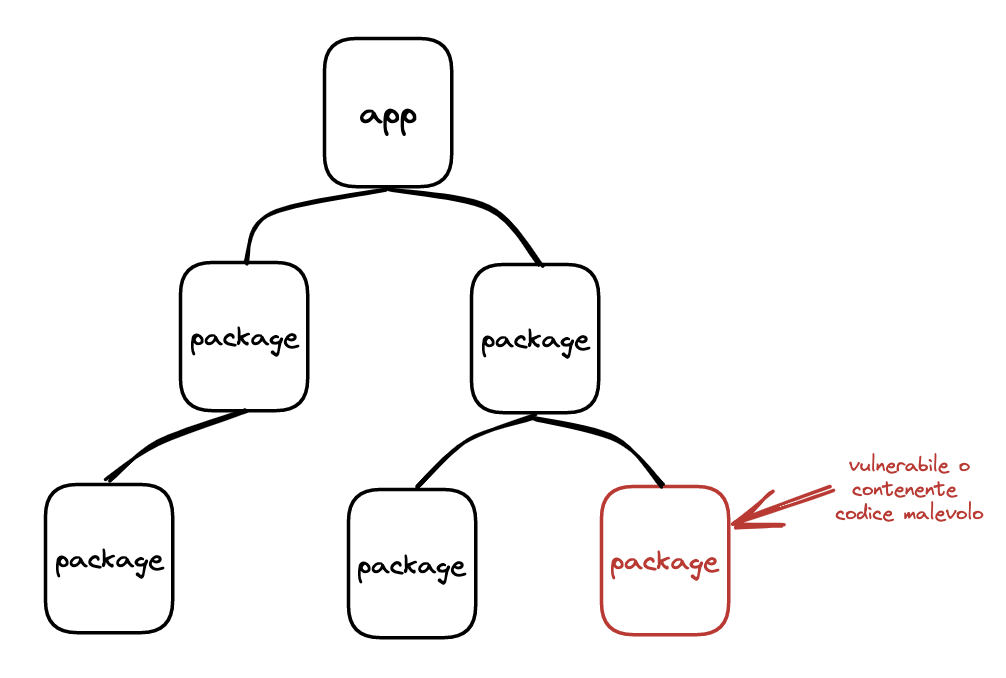
\includegraphics[width=8cm]{./chapters/2.wasi-in-depth/images/1.malicious_or_vuln_code.png}
    \label{app_package}
    \caption{Come sono composte le applicazioni moderne}
\end{figure}
In questo modo, è possibile ridurre il lavoro necessario per la creazione di applicazioni complesse, migliorare
l'efficienza del processo di sviluppo e aumentare la qualità del software prodotto. D'altra parte, questo modello di
sviluppo espone le applicazioni ad una grossa problematica, cosa succederebbe se in uno di questi pacchetti software ci
fosse inserito codice malevolo o codice vulnerabile? Purtroppo non è uno scenario remoto:
\begin{quote}
    The average application development project has 49 vulnerabilities and 80 direct dependencies (open source code
    called by a project); \\
    \textit{Snyk 2019 State of Open Source Security
    Report}\footnote{\url{https://snyk.io/reports/open-source-security/}}
\end{quote}
Per peggiorare le cose, non tutte queste vulnerabilità vengono risolte, si stima che solo il 59\% dei pacchetti software
risolva le vulnerabilità trovate.
\subsection{Una possibile soluzione}
Esistono diverse strategie che gli sviluppatori possono adottare per proteggere il loro software e gli utenti finali. Ad
esempio, si potrebbe utilizzare uno scanner per controllare le applicazioni e le dipendenze, tuttavia questa soluzione
non è sempre efficace, poiché gli scanner sono facilmente aggirabili. Un'altra opzione potrebbe essere quella di
registrarsi ad un servizio che notifichi gli sviluppatori delle vulnerabilità trovate nel codice, ma anche questa
soluzione presenta delle limitazioni, in quanto potrebbe non individuare tutte le vulnerabilità presenti nel software.
Infine, un'altra strategia possibile sarebbe quella di revisionare il codice ogni volta che si fa un update delle
dipendenze, ma questa soluzione potrebbe funzionare solo per progetti piccoli con poche dipendenze, mentre per progetti
più grandi e complessi potrebbe risultare impraticabile. Le soluzioni esistenti cercano di individuare le vulnerabilità
del software, ma non offrono una vera e propria prevenzione. La soluzione ideale sarebbe quella di prevenire le
vulnerabilità alla radice. Per arrivare alla soluzione, dobbiamo tornare un po' indietro nel tempo, in quanto è un
problema già affrontato in passato, solo con un altro tipo di granularità. \\
\\
Il problema di far coesistere due applicazioni in esecuzione senza interferenze reciproche esiste fin dai primi sistemi
operativi. La soluzione adottata è affidare al sistema operativo il compito di proteggere e controllare l'esecuzione
delle applicazioni tramite l'utilizzo dei "processi". Quando una nuova applicazione viene avviata, il sistema operativo
crea un nuovo processo con un'area di memoria dedicata, che non può accedere alle aree riservate degli altri processi.
Se il processo ha bisogno di comunicare con altri, deve prima richiedere il permesso e farlo tramite le "pipe".
\begin{figure}[h]
    \centering
    \captionsetup{justification=centering}
    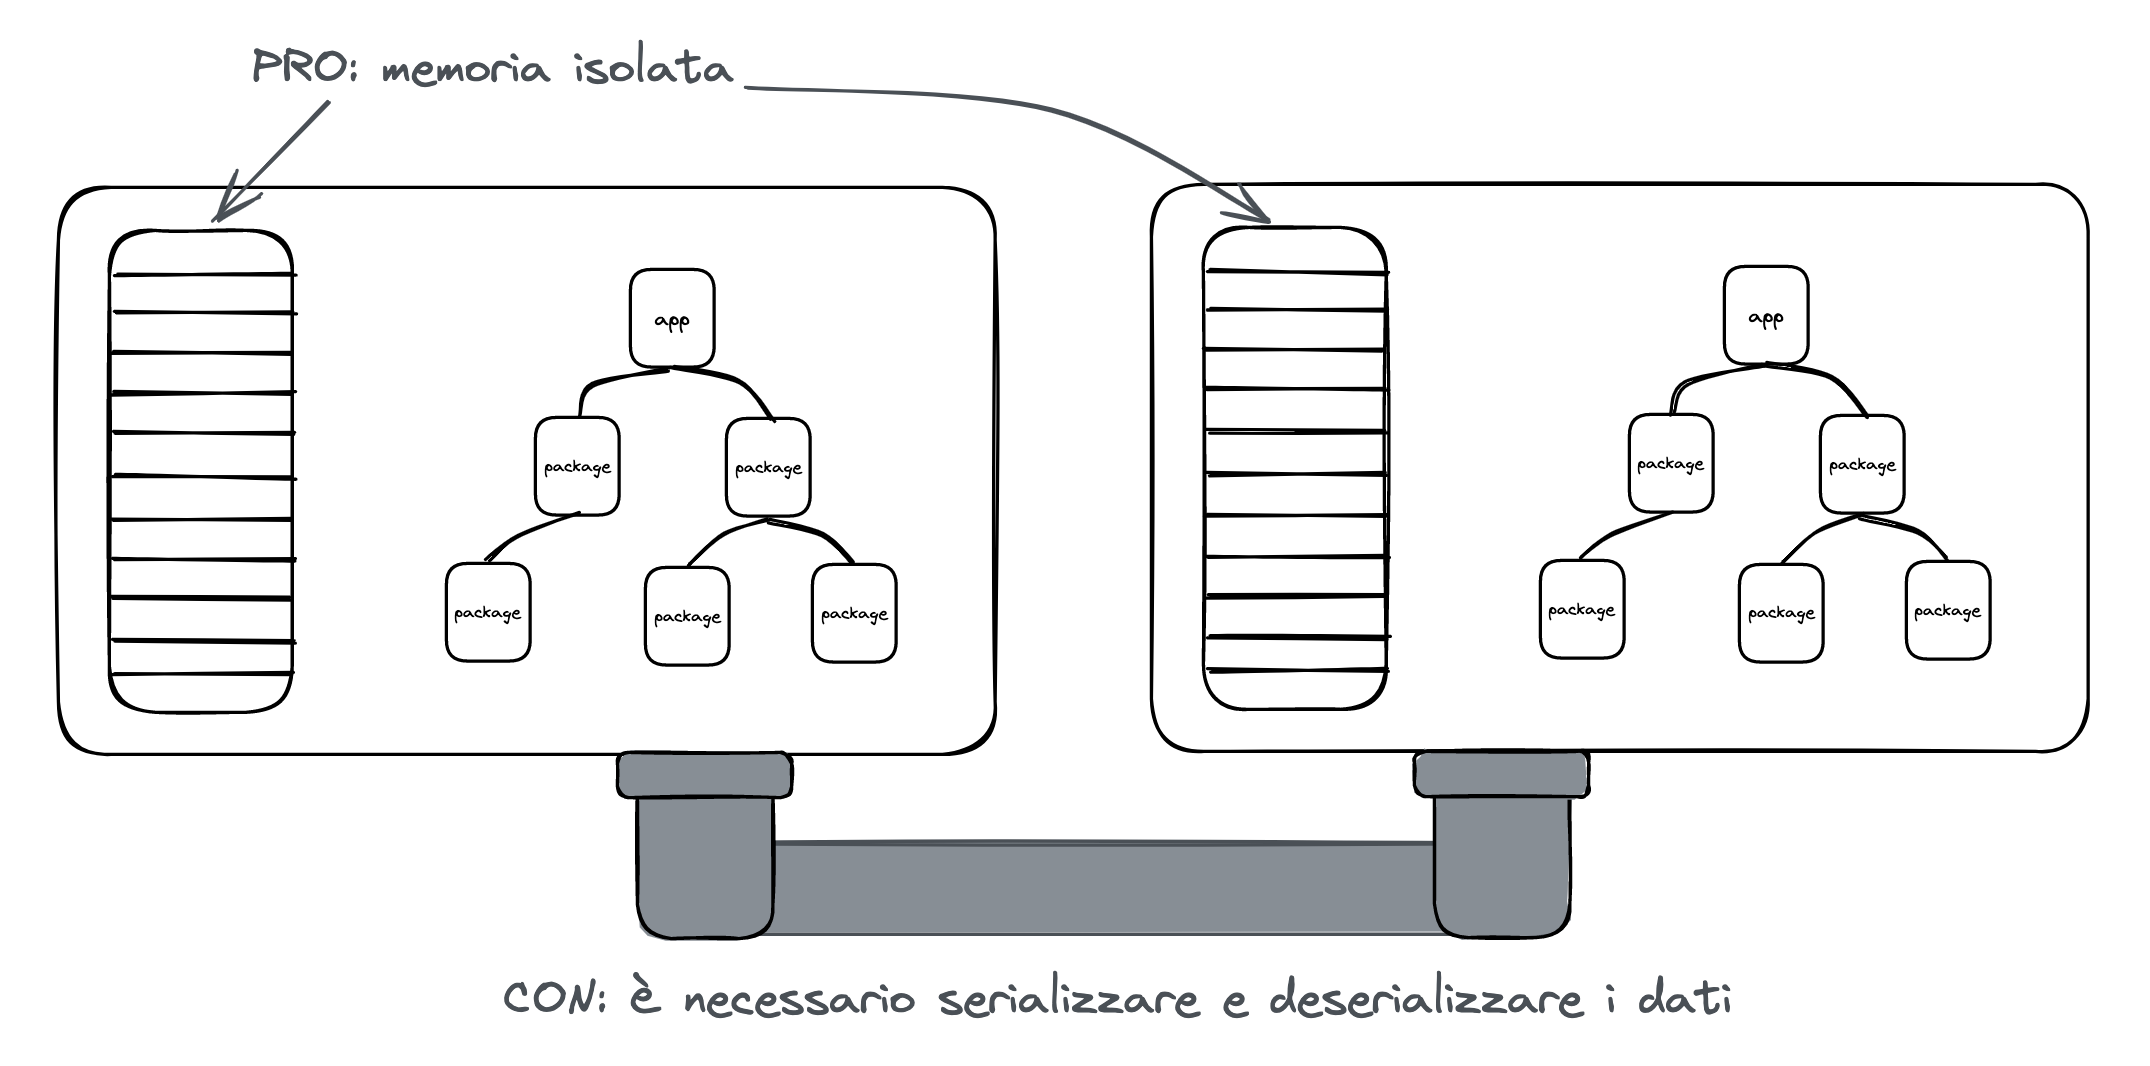
\includegraphics[width=10cm]{./chapters/2.wasi-in-depth/images/2.process_isolation.png}
    \label{process_isolation}
    \caption{Isolamento dei processi nei sistemi operativi}
\end{figure}
Questo sistema risolve il problema della condivisione della memoria a runtime, ma non garantisce che l'applicazione, ad
esempio, non acceda al filesystem per effettuare qualche operazione non prevista.\\ 
Le VM e i container sono stati sviluppati in origine proprio per questo motivo, garantiscono che qualcosa in esecuzione
in una VM o container non possa accedere al filesystem di altri, ma non nel proprio. Con il modello "sandbox", invece,
potremmo ulteriormente isolare le applicazioni rimuovendo l'accesso alle API e alle system call del sistema prima che
l'applicazione venga eseguita. Guardando alle tre soluzioni potremmo arrivare alla conclusione che per garantire la
sicurezza e l'isolamento di ogni package sia necessario isolarlo all'interno della propria sandbox, con i giusti
permessi. Ciò però porterebbe presto ad un esaurimento delle risorse del sistema ed introdurrebbe un overhead nella
comunicazione tra i package dell'applicazione. 
\begin{figure}[H]
    \centering
    \captionsetup{justification=centering}
    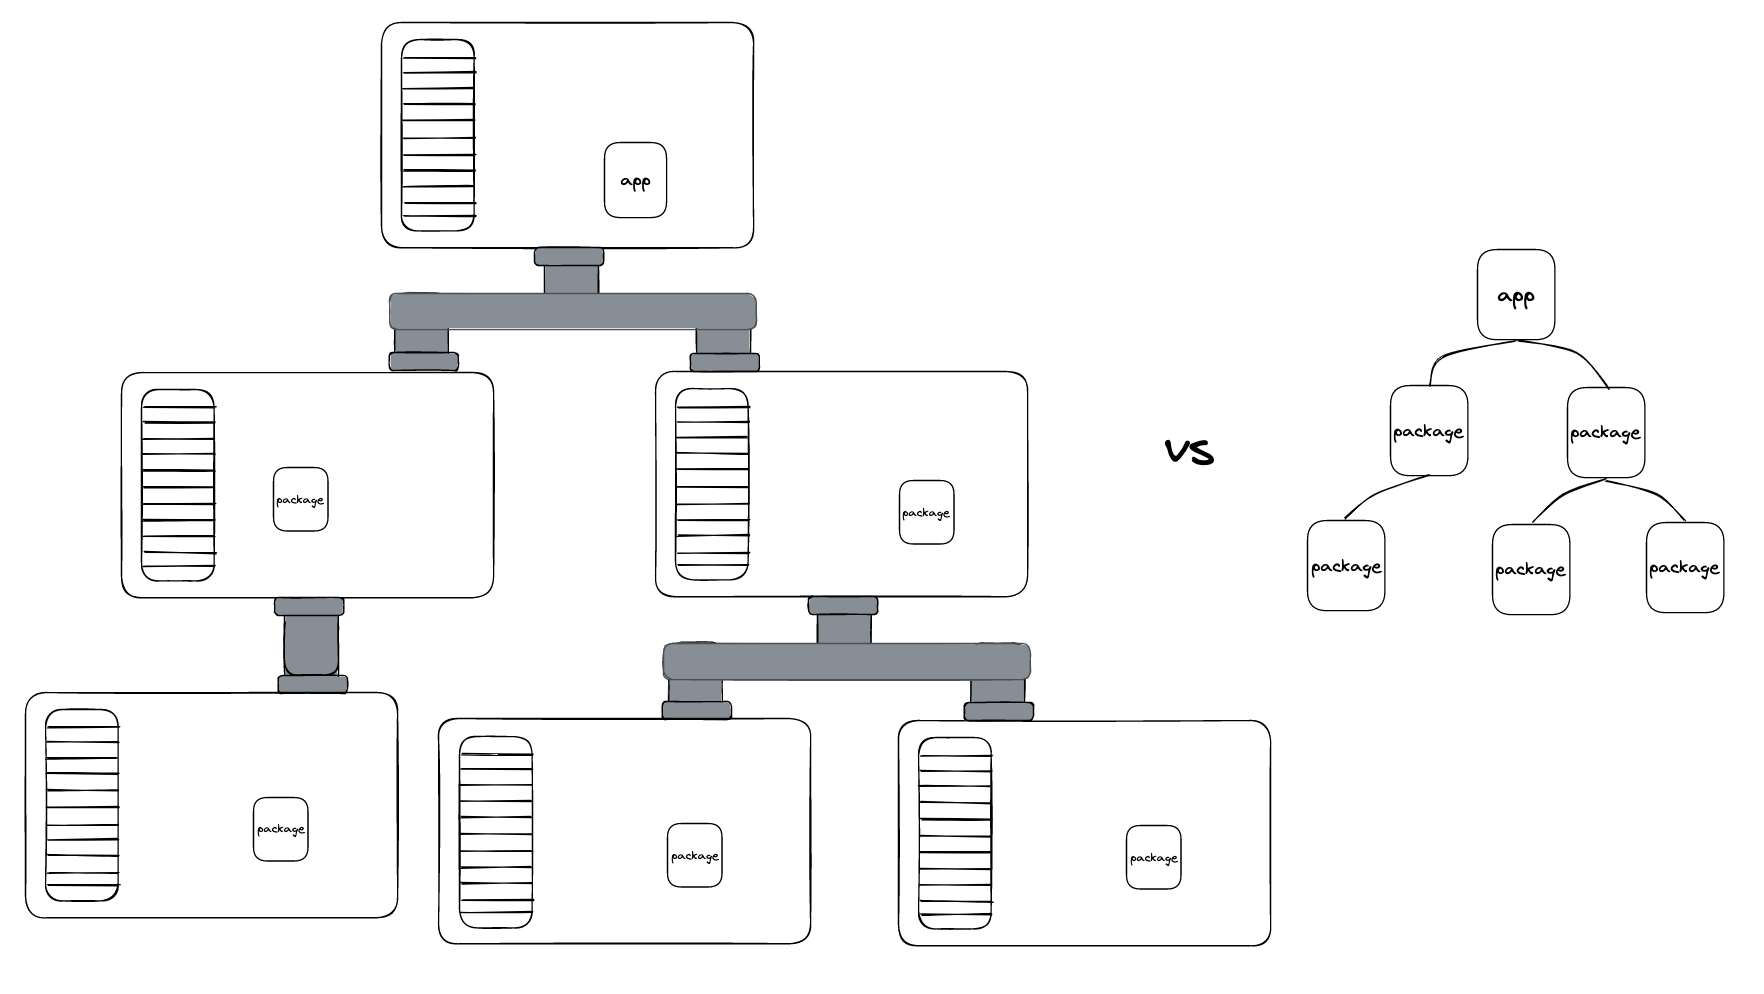
\includegraphics[width=10cm]{./chapters/2.wasi-in-depth/images/3.package_isolation_processes.png}
    \label{process_package_in_sandbox}
    \caption{Isolamento dei package in sandbox isolate, evidente inefficienza e overhead}
\end{figure}
Come facciamo quindi a garantire l'isolamento di ogni package senza esaurire le risorse del sistema?
\subsection{La soluzione: nanoprocessi}
WebAssembly offre un'efficace forma di isolamento che previene al codice non sicuro di fare ciò che vuole, i
nanoprocessi. I nanoprocessi sono strutture simili ai processi standard di Unix ma che risultano essere più leggeri e di
dimensioni ridotte. Risiedono all'interno di un ambiente di esecuzione chiamato "sandbox", che rappresenta un processo
padre isolato dall'esterno. La memoria a cui ogni nanoprocesso ha accesso è uno slice della memoria del processo padre,
ovvero della sandbox. Per accedere ai dati di un altro modulo, un modulo deve avere l'autorizzazione esplicita per farlo
e questa autorizzazione viene passata in modo gerarchico, dall'alto verso il basso. In questo modo, la sandbox coordina
l'accesso ai dati e garantisce che ogni nanoprocesso operi in modo indipendente e sicuro, senza che vadino ad
interferire con gli altri. L'uso di nanoprocessi consente di ottimizzare le prestazioni dell'applicazione, evitando
costose chiamate di sistema e semplificando la comunicazione tra i vari moduli Wasm.
\begin{figure}[h]
    \centering
    \captionsetup{justification=centering}
    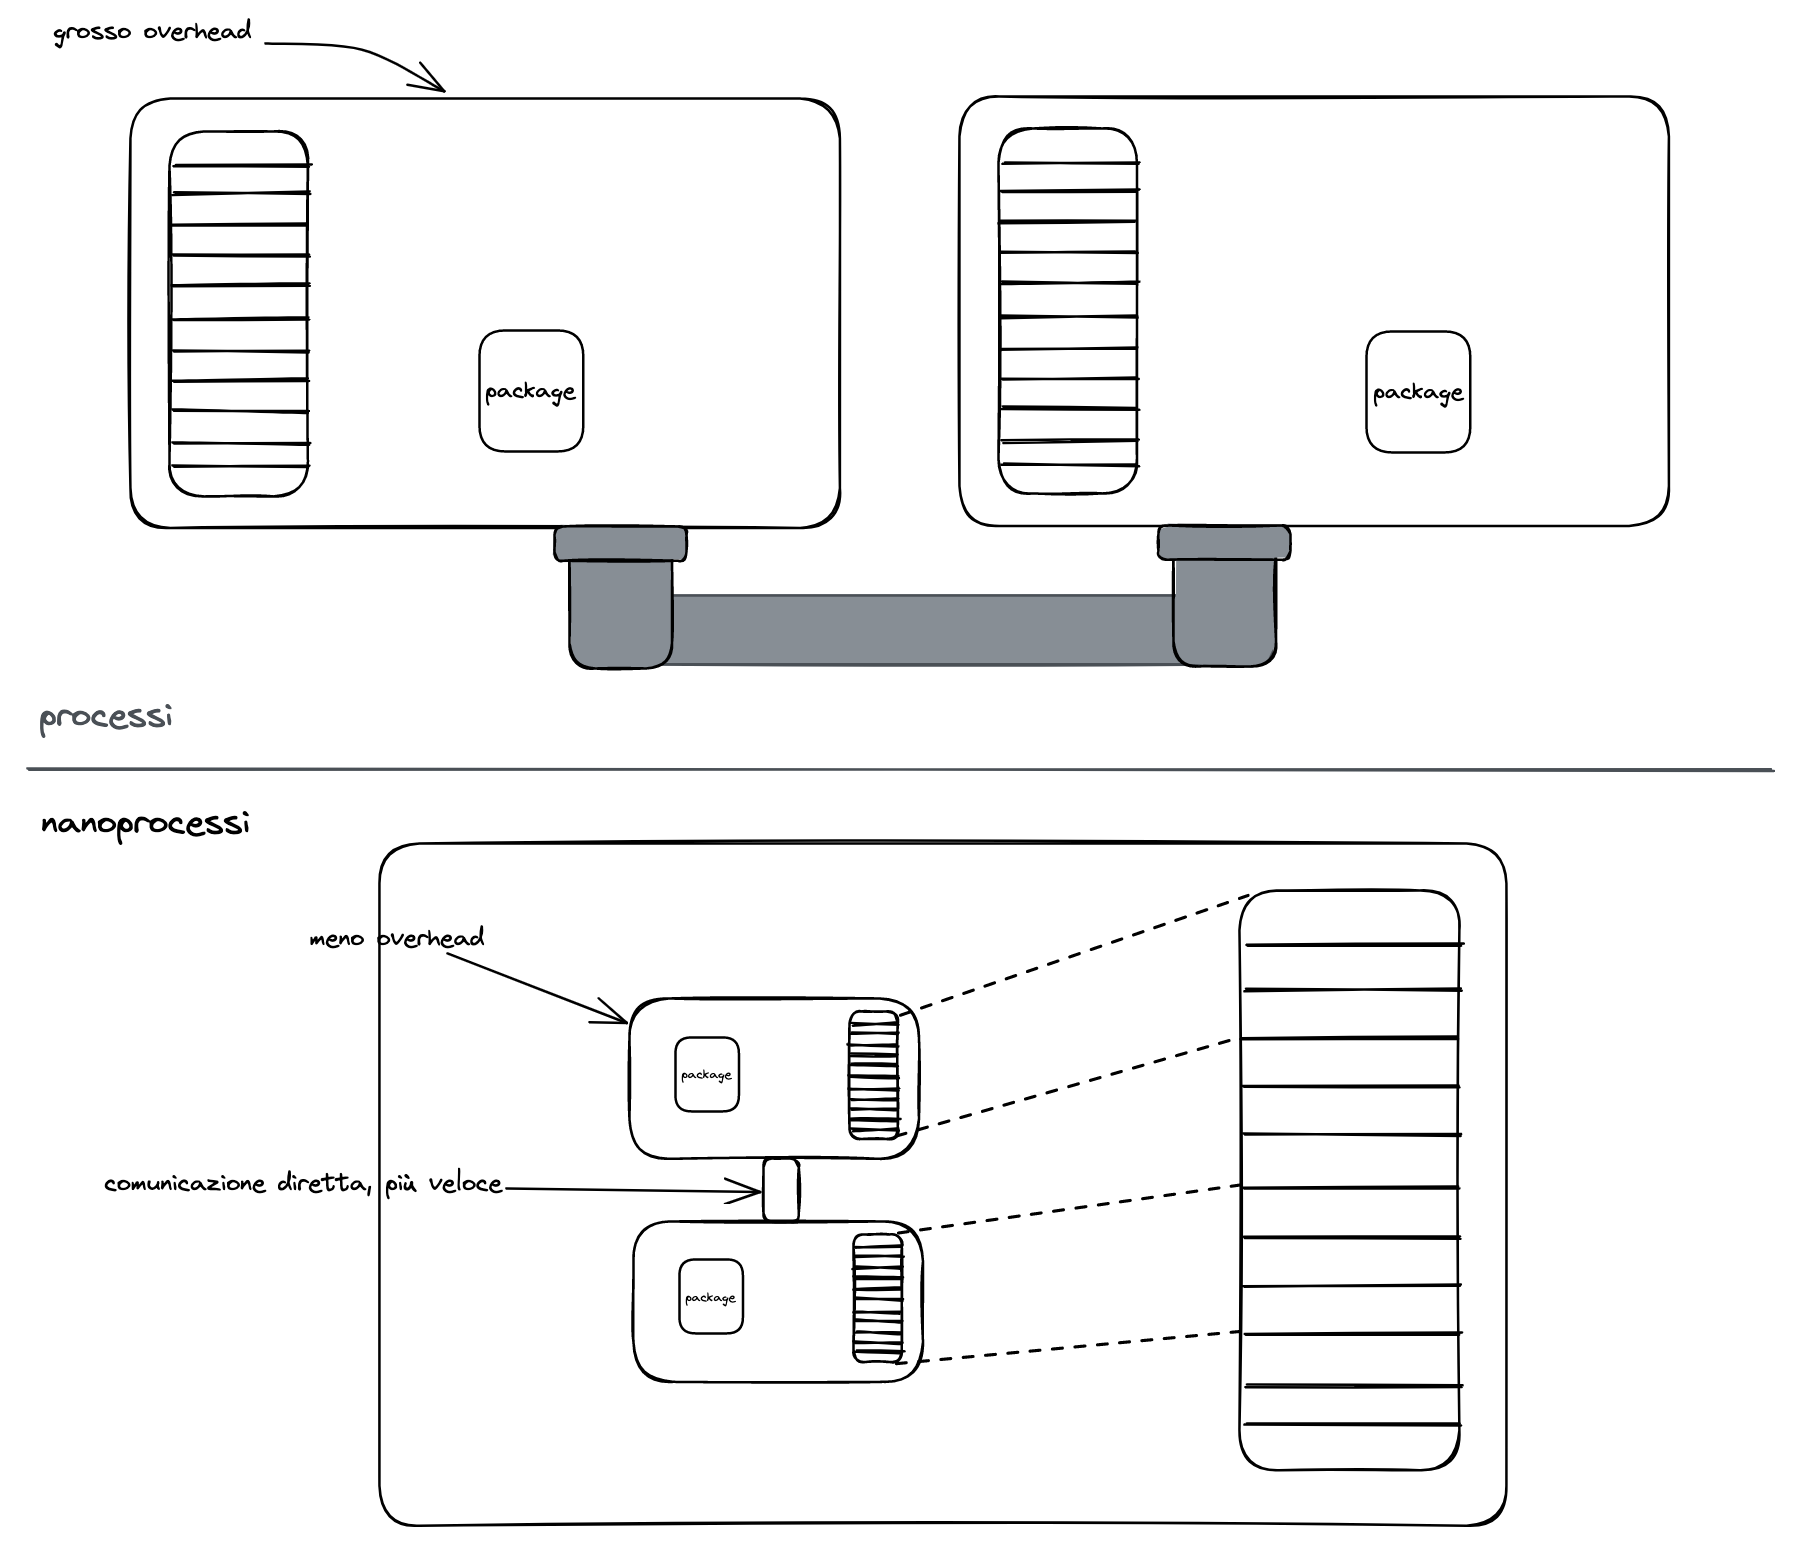
\includegraphics[width=10cm]{./chapters/2.wasi-in-depth/images/4.nanoprocesses.png}
    \label{nanoprocesses}
    \caption{Nanoprocessi di Wasm}
\end{figure}
Si noti che il concetto di nanoprocesso in WebAssembly è basato sui processi Unix, ma implementato attraverso un pattern
specifico di WebAssembly.\\
Tutte le caratteristiche di WebAssembly descritte finora rendono questa tecnologia una soluzione sicura per l'esecuzione
di codice al di fuori del browser. Per esempio, se del codice malevolo tentasse di accedere a un file su cui la sandbox
non ha i permessi, il modulo WebAssembly verrebbe interrotto sollevando un'eccezione e il processo finirebbe con un
errore. Inoltre, anche se la sandbox avesse i permessi per accedere a un determinato file, questi permessi potrebbero
non essere associati al modulo contenente il codice malevolo. In relazione al codice vulnerabile, sarebbe estremamente
difficile per un attaccante trovare un modulo che abbia sia l'autorizzazione a utilizzare una determinata system call
sia l'autorizzazione su un determinato file nel filesystem. \\ Si può notare come questa filosofia di WebAssembly
aderisca al principio di least authority (POLA) e al capability based model.
\subsection{Capability Based Model}
Il modello basato sulle capacità è un approccio alla sicurezza che si basa sulla concessione di autorizzazioni
specifiche, chiamate "capacità", ai processi del sistema, concepito a metà degli anni
sessanta\cite{capability-based-security}. È un'alternativa alle ACL (Access Control List) che sono un metodo di
controllo degli accessi basato su liste di controllo degli accessi, dove ogni oggetto (come file, cartelle, stampanti,
ecc.) ha una lista di controllo degli accessi associata che contiene una serie di voci per specificare quali utenti o
gruppi hanno il permesso di accedere all'oggetto e quali tipi di accesso sono consentiti (come lettura, scrittura,
esecuzione, ecc.). In un modello di sicurezza basato su capability, ogni processo ha un insieme di capacità specifiche
che gli consentono di accedere alle risorse del sistema. Una capacità non è altro che una chiave di autorità, associata
ad un particolare oggetto. Possiamo pensarla come un indice che punta ad una tupla (x, r), dove x è l'oggetto ed r è
l'insieme dei diritti d'accesso su di esso. Ad esempio, se la tupla (file1, \{leggi, scrivi\}) è associata ad un
processo tramite una reference mantenuta da questo, tale processo può leggere e scrivere sul file1, ma non può eseguire
altre azioni su di esso. Quando un processo deve accedere all'oggetto, può farlo senza richiedere l'autorizzazione al
sistema operativo, in quanto il possesso della capability (la reference) rappresenta già l'autorizzazione per farlo. In
un modello basato sulle capabilities, il sistema operativo non è responsabile del controllo delle autorizzazioni per i
processi, ma piuttosto della gestione della lista di capabilities disponibili e della prevenzione di eventuali modifiche
non autorizzate.
\subsubsection{Un esempio}
Supponiamo che un processo abbia in memoria il seguente path:
\begin{lstlisting}
    /etc/shadow
\end{lstlisting}
Questo rappresenta il nostro oggetto della tupla e supponiamo poi di aver associato all'oggetto anche il permesso di
lettura: 
\begin{lstlisting}
    O_RDWR
\end{lstlisting}
Così da avere la tupla (/etc/shadow, O\_RDWR). Questa non rappresenta ancora la capability per il processo di accedere
all'oggetto poiché non si può verificarne l'autorità su di esso. Ipotizziamo ora di avere anche il file descriptor per
tale file.
\begin{lstlisting}
    int fd = open("/etc/shadow", O_RDWR);
\end{lstlisting}
La variabile fd contiene l'indice di un descrittore di file presente nella tabella dei descrittori di file del processo,
che rappresenta la capability dell'oggetto a cui si sta accedendo. La presenza di questo descrittore nella tabella dei
descrittori è sufficiente per garantire che il processo abbia accesso legittimo all'oggetto. \\

WASI adotta il modello di Nuxi CloudABI\footnote{\url{https://github.com/NuxiNL/cloudabi}}, che unisce i concetti di
POSIX e del modello capability based. In questo modello, ogni risorsa del sistema, come file, directory e socket, è
identificata da un file descriptor UNIX-like, che rappresenta la capability su un certo oggetto del sistema. Ciò
significa che un processo non può accedere a tale oggetto se non è in possesso della capability adatta. Per esempio,
WASI non permette l'accesso alla system call open() che restituisce un file descriptor, ma al contrario, utilizza la
opennat system call, che richiede un file descriptor precedentemente aperto, ovvero la capability. Essenzialmente
quindi, un modulo Wasm potrà interagire, ad esempio con il filesystem, solo se la sandbox gli fornirà in precedenza le
capabilities necessarie su di una certa directory all'avvio. Questi file descriptor saranno aperti in anticipo dalla
sandbox tramite la \hyperref[sec:libpreopen]{Libpreopen} e passati ai moduli Wasm quando necessario.
\subsubsection{Il modello in azione: un esempio}
Per comprendere meglio questo modello, possiamo analizzare un'applicazione scritta in
Rust\footnote{\url{https://github.com/ilcors-dev/bachelor-thesis/tree/main/prototypes/1.file}} che si occupa di copiare
dei file del filesystem. Per eseguire il modulo Wasm generato dalla compilazione del codice sorgente, utilizzeremo
Wasmtime come runtime.
\begin{figure}[H]
    \centering
    \captionsetup{justification=centering}
    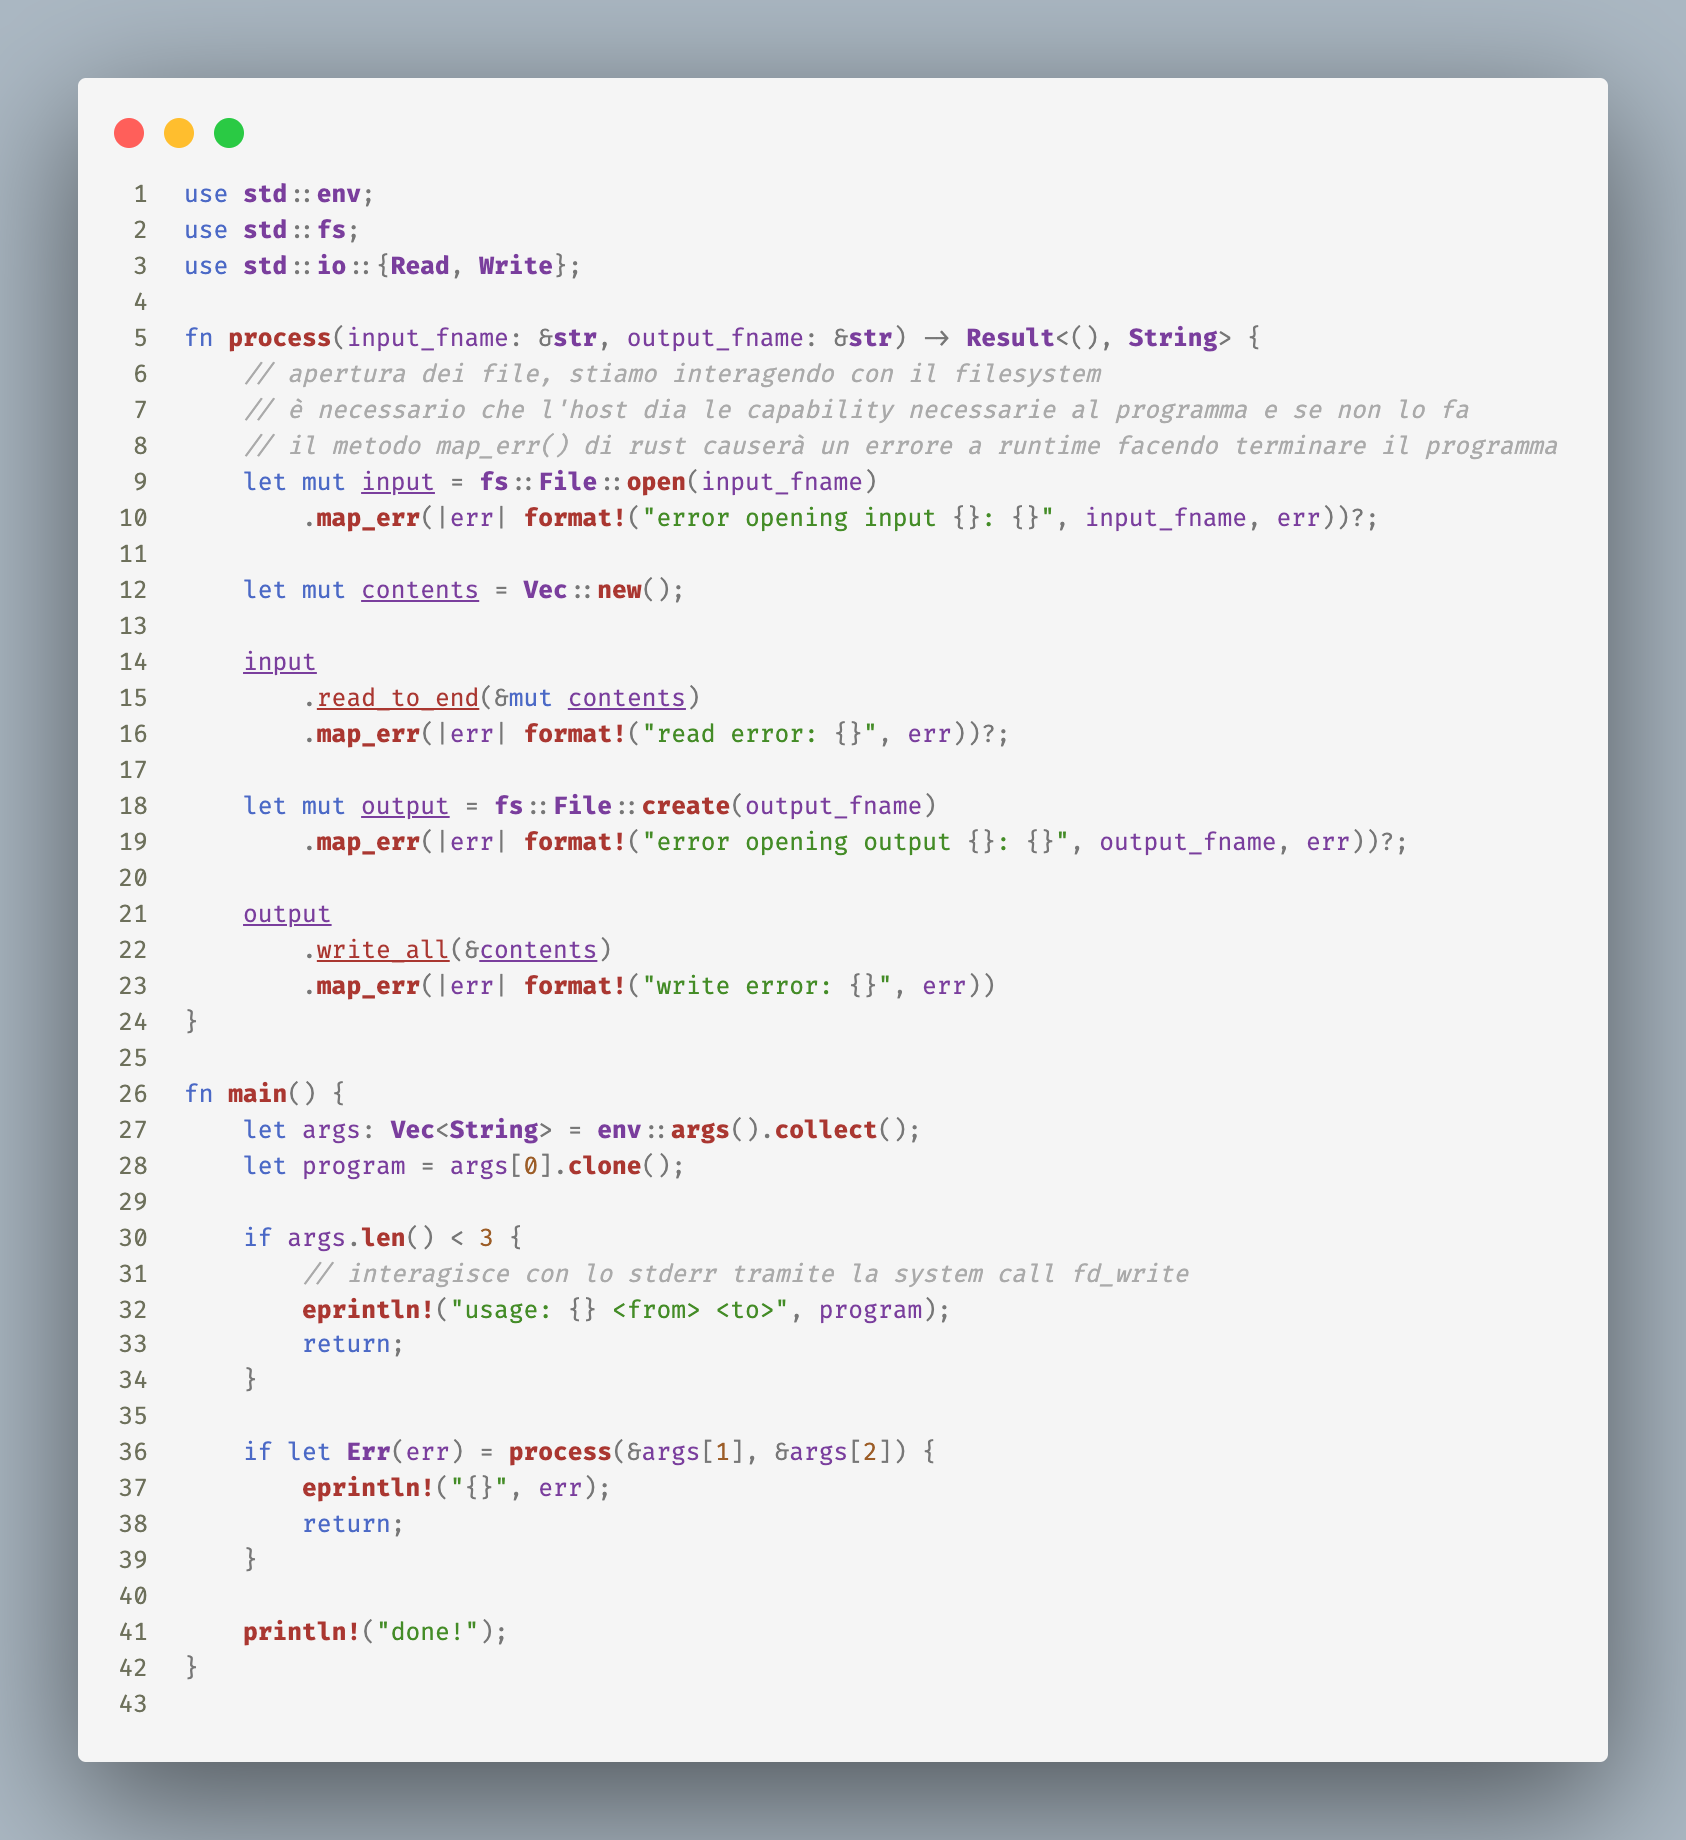
\includegraphics[width=15cm]{./chapters/2.wasi-in-depth/images/5.wasi_capability_example.png}
    \label{wasi_capabilities_example}
    \caption{Il modello capability based in azione}
\end{figure}
Compilando il programma tramite cargo, il gestore di pacchetti predefinito di Rust.
\begin{lstlisting}
    cargo build --target wasm32-wasi
\end{lstlisting}

Proviamo ad eseguire il programma senza garantire le capability necessarie con Wasmtime.

\begin{lstlisting}
    wasmtime target/wasm32-wasi/debug/file.wasm tocopy.txt /tmp/out.txt
    error opening input tocopy.txt: failed to find a pre-opened file descriptor through which "tocopy.txt" could be opened
\end{lstlisting}
Cosa è andato storto? Analizzando l'errore, si evince che il programma sta tentando di aprire un file chiamato
'tocopy.txt', ma non dispone del file descriptor necessario per farlo. In altre parole, Wasmtime non ha
fornito le capability adatte per consentire all'applicazione di eseguire questa operazione.
\\
Proviamo invece a fornire le giuste capability al programma in questo modo:
\begin{lstlisting}
    wasmtime --dir=. --dir=/tmp target/wasm32-wasi/debug/file.wasm tocopy.txt /tmp/out.txt
    done!
\end{lstlisting}
Analizziamo cosa sta succedendo. L'opzione --dir istruisce Wasmtime di pre-aprire la cartella corrente '.' e la cartella
di destinazione /tmp rendendole entrambi disponibili al programma. Quando l'applicazione chiama la funzione File::open
sta effettivamente chiamando la system call open() passando come parametro il path del file. In questo frangente
interviene la WASI libc, che in modo trasparente, traduce il path in un path relativo a quello già pre-aperto in
precedenza da Wasmtime utilizzando la libreria \hyperref[sec:libpreopen]{Libpreopen}. \\In questo modo WASI è in grado
di adottare il modello capability based e portarlo a livello di system call senza che il programma in sè debba essere
modificato!

È importante notare che, di default, la sandbox non espone la variabile d'ambiente \$PWD all'applicazione WebAssembly,
la directory corrente va pertanto passata attraverso un path relativo. Infatti:
\begin{lstlisting}
    wasmtime --dir=\$PWD --dir=/tmp target/wasm32-wasi/debug/file.wasm tocopy.txt /tmp/out.txt
    error opening input tocopy.txt: failed to find a pre-opened file descriptor through which "tocopy.txt" could be opened
\end{lstlisting}

E i path traversal? Funzionano? Sappiamo che in applicazioni
tradizionali la sanificazione dell'input è a carico dello sviluppatore, mentre con WASI?

\begin{lstlisting}
    wasmtime --dir=. --dir=/tmp target/wasm32-wasi/debug/file.wasm tocopy.txt /tmp/../etc/passwd
    error opening output /tmp/../etc/passwd: failed to find a pre-opened file descriptor through which "/tmp/../etc/passwd" could be opened
\end{lstlisting}

Come possiamo notare l'applicazione viene bloccata prima di raggiungere il sistema operativo, infatti l'errore non
riguarda gli eventuali permessi necessari per accedere ad /etc/passwd, bensì parla della mancanza di capacità necessaria
per effettuare l'operazione. Le applicazioni WASI non hanno possibilità di accedere a file al di fuori delle directory
esplicitamente garantite dalla sandbox!

In conclusione, possiamo affermare che WASI adotta una metodologia di sicurezza estremamente robusta grazie al modello
di least authority e al principio di capability. Ciò si traduce in applicazioni molto più sicure di default grazie alla
riduzione della superficie di attacco disponibile.
\subsubsection{Il problema delle socket}
\section{La gestione delle risorse}

\section{Portabilità}
\section{Nei container}